\section{Auswertung}

Die für die Auswertung notwendige Regressionsrechnung wurde mit Hilfe
des Paketes curve\_fit erstellt.

Die Rubidium-Isotope $\ce{^{85}Rb}$ und $\ce{^{87}Rb}$ werden im Laufe der Auswertung
bestimmt. Bevor die Identifikation stattfindet werden die Messdaten, die zu
der ersten Resonanzstelle gehören mit einer eins indiziert und die Messdaten, die
zu der zweiten gehören mit einer zwei.

Ein typisches Signalbild des Versuches ist in Abbildung \ref{fig:typisch}
dargestellt.

\begin{figure}[h]
  \centering
  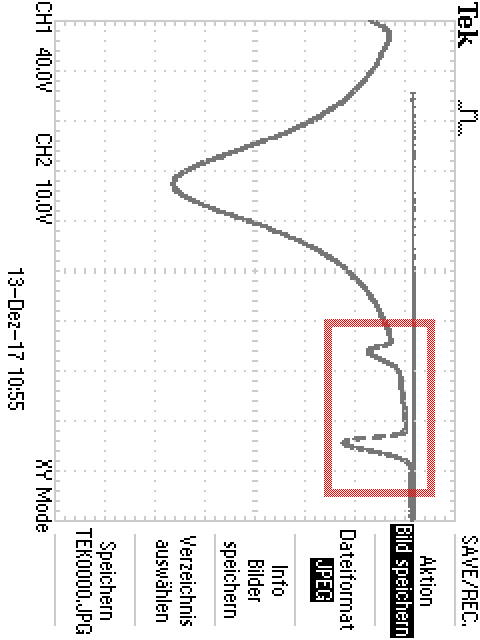
\includegraphics[angle = 90]{Pics/edit_typical.jpg}
  \caption{Typisches Signalbild}
  \label{fig:typisch}
\end{figure}

In Abbildung \ref{fig:typisch} sind die beiden Resonanzstellen in dem schraffierten
Rechteck zu erkennen.

\subsection{Erdmagnetfeld}

Der Tisch mit dem darauf befindlichen Versuchsaufbau ist so ausgerichtet, dass nur die
Horizontalkomponente des Erdmagnetfeldes Einfluss auf den Versuch hat.
Die Helmholtzspule, die diese Horizontalkopmonente kompensiert bestand aus
20 Windungen die einen mittleren Radius von $R\ua{vertikal} = \SI{11.735}{\centi\meter}$ besitzen.
Die Spule kompensiert ab einen eingestellten Strom von $I\ua{vertikal} = \SI{0.23}{\ampere}$ das
Erdmagnetfeld.
Durch die Formel für Helmholtzspulen

\begin{equation}
  \label{eqn:helmholtz}
  B\ua{Spule} = \mu_0\cdot\frac{8\cdot I\cdot N}{\sqrt{125}\cdot R}
\end{equation}

berechnet sich die Horizontalkomponente des Erdmagnetfeldes zu $B\ua{Erd} = \SI{0.0349}{\milli\tesla}$.

\subsection{Bestimmung der Landé-Faktoren und des Kernspins der Rubidium--Isotope}

Die Landé-Faktoren $g_{F_i}$ lassen sich durch eine Lineareregression mit der Formel \ref{eqn:Bm}
ermitteln. Die Messdaten der Frequenzen und den zugehörigen gemessenen Stromstärken sind
in den Tabellen \ref{tab: Messdaten_Resonanz_1} und \ref{tab: Messdaten_Resonanz_2} dargestellt.
Eine Darstellung der linearen Regression ist
in \ref{fig:regression} abgebildet.

\begin{figure}[h]
  \centering
  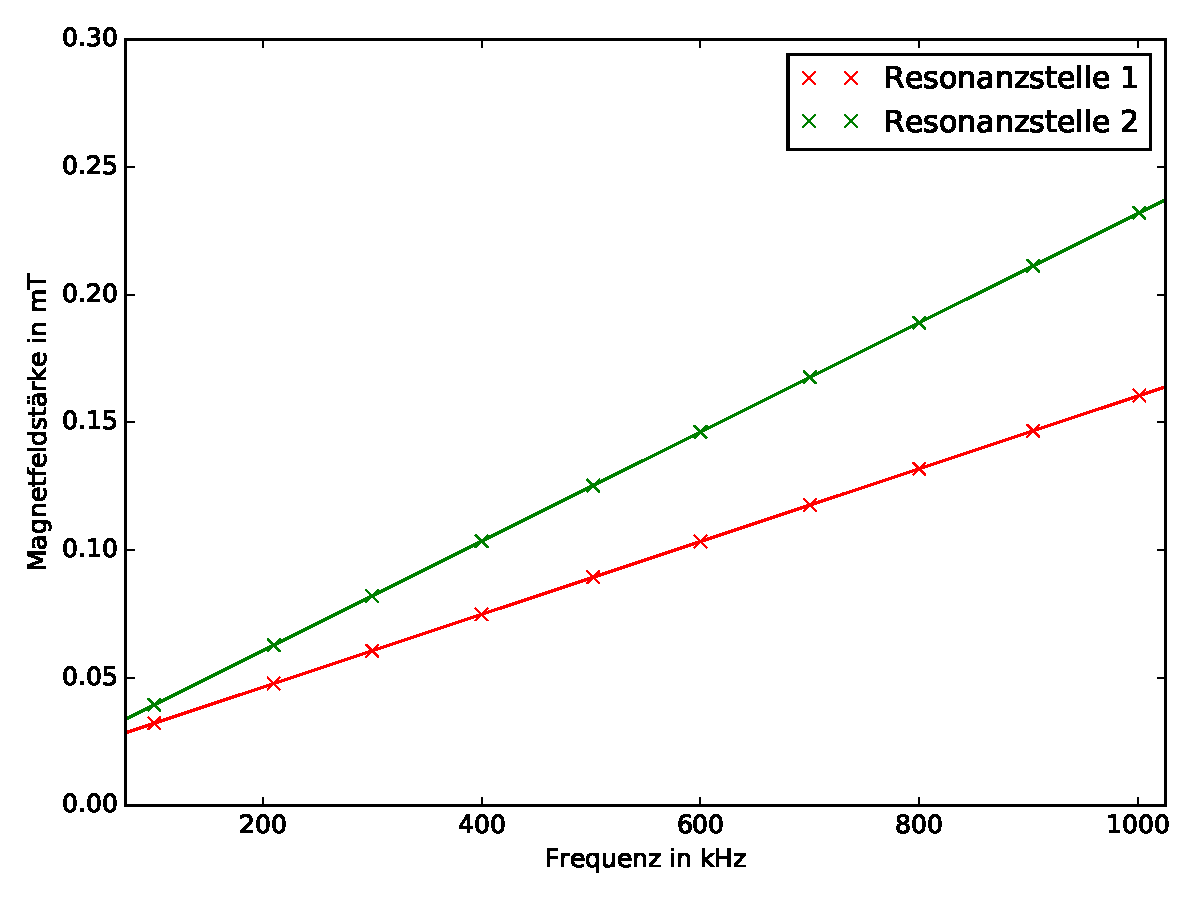
\includegraphics[width = \textwidth]{Python/frequenz_B_feld.pdf}
  \caption{Lineare Regression der B-Feldstärken an den Resonanzstellen mit steigender Frequenz}
  \label{fig:regression}
\end{figure}

Die Landé-Faktoren der Isotope sind wie folgt.

\begin{align*}
  g\ua{F_1} &= \num{0.5011(19)} \\
  g\ua{F_2} &= \num{0.3339(11)}
\end{align*}

Die Rubidium-Isotope haben die folgenden Quantenzahlen.

\begin{align*}
  L = 0, \qquad
  S = \frac{1}{2}, \qquad
  J = \frac{1}{2} \\
\end{align*}

Mit den obigen Quantenzahlen ist $g\ua{J} = \num{2.0023}$.

Somit kann unter Berücksichtigung von $F = I + J$ Formel \ref{eqn:g_F} nach $I$
umgestellt werden.

\begin{equation}
  \label{eqn:Kernspin}
  I = \frac{g\ua{J}}{4g\ua{F}} - 1 + \sqrt{\left(\frac{g\ua{J}}{4g\ua{F}} - 1\right)^2 + \frac{3}{4}\left(\frac{g\ua{J}}{g\ua{F}} - 1\right)}
\end{equation}

Die Kernspins der Rubidium-Isotope ergeben sich zu:

\begin{align*}
  I_1 &= \num{1.498(7)} \\
  I_2 &= \num{2.498(10)}.
\end{align*}

Damit wird erkenntlich, dass die erste Resonanzstelle zu dem Isotop $\ce{^{87}Rb}$
und die zweite Resonanzstelle zu dem Isotop $\ce{^{85}Rb}$ gehört.

\subsection{Isotopenverhältnis}

Aus der Abbildung \ref{fig:Resonanzstellen} sind die Amplituden der beiden
Resonanzstellen zu entnehmen.
Das Isotopenverhätnis $R = \frac{p_1}{p_2}$ ergibt sich aus den Amplitudenverhältnis.
In der Versuchkammer liegen $p_1$ Anteile von $\ce{^{87}Rb}$ und $p_2$ Anteile
von $\ce{^{85}Rb}$ vor. Insgesamt gilt $p_1 + p_2 = 1$.
Somit folgt, dass $p_2 = \frac{1}{1 + R}$ ist.

\begin{align*}
  R &= 44,5 \\
  p_1 &= 30,81 \% \\
  p_2 &= 69,19 \% \\
\end{align*}

\begin{figure}[h]
  \centering
  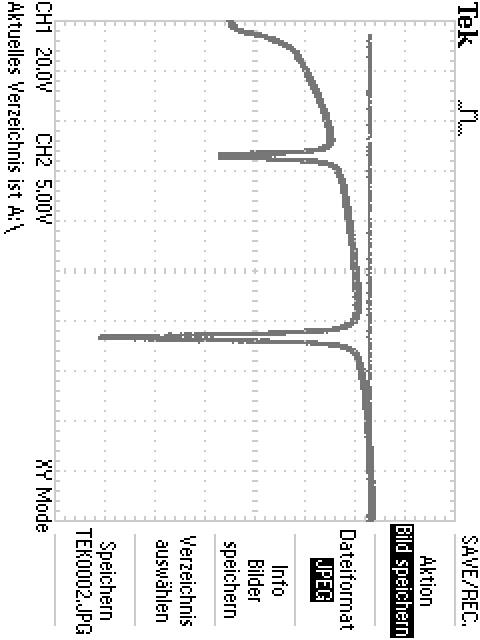
\includegraphics[angle = 90]{Pics/TEK0002.JPG}
  \caption{Nahaufnahme der beiden Resonanzstellen}
  \label{fig:Resonanzstellen}
\end{figure}

\subsection{Quadratischer Zeeman-Effekt}

Mit Formel \ref{eqn:Uneu} lässt sich der quadratische Zeeman-Effekt abschätzen und mit dem
linearen Term vergleichen.

Für das Rubidium-Isotope werden die folgenden Daten verwendet.
Dabei sind für die B-Felder die Werte an den Resonanzen gemittelt über alle gemessenen Werte angenommen worden.

\begin{align*}
  \ce{^{87}Rb}: &\\
  B &= \SI{9.65e-2}{\milli\tesla} \\
  \symup{M}\ua{F} &= 2 \\
  \Delta E\ua{Hy} &= \SI{4.53e-24}{\joule}\\
  \\
  \ce{^{85}Rb}: &\\
  B &= \SI{0.136}{\milli\tesla} \\
  \symup{M}\ua{F} &= 3 \\
  \Delta E\ua{Hy} &= \SI{2.01e-24}{\joule}
\end{align*}

\newpage

Damit ergeben sich die Terme der Hyperfeinstrukturaufspaltung zu:

\begin{description}
  \item[$\ce{^{87}Rb}$]
  \item[Linear] $\SI{4.483(17)e-28}{\joule}$
  \item[Quadratisch] $\SI{-1.331(10)e-31}{\joule}$
  \\
  \item[$\ce{^{85}Rb}$]
  \item[Linear] $\SI{4.209(13)e-28}{\joule}$
  \item[Quadratisch] $\SI{-4.407(28)e-31}{\joule}$
\end{description}




\section{Diskussion}

In der Auswertung sind keine Ablesefehler der Spulenströme berücksichtigt worden,
wordurch die Aussagekraft der Ergebnisse verringert wird.

Im Allgemeinen spiegeln jedoch die erhobenen und ausgewerteten Ergebnisse in guter Näherung die
Literatruwerte wieder. Der Kernspin des Rubidium-Isotopes $\ce{^{85}Rb}$ wird in der Literatur
mit einem Wert von $I\ua{Literatur} = \frac{5}{2}$ angegeben. Die Auswertung der Messdaten ergab
einen Kernspin von $I_{\ce{^{85}Rb}} = \num{2.498(10)}$. Der Literaturwert liegt somit
in der Fehlerschranke und konnte hier experimentell bestätigt werden.
Gleiches gilt für den Kernspin des Isotopes $\ce{^{87}Rb}$. Der zugehörige
Literaturwert beträgt $I\ua{Literatur} = \frac{3}{2}$ und wurde im Experiment mit
$I_{\ce{^{87}Rb}} = \num{1.498(7)}$ wieder gefunden.
Die Kernspins stimmen somit mit den Literaturwerten nahezu überein, weshalb angenommen wird,
dass die berechneten Landé-Faktoren   $g\ua{F_1} = \num{0.5011(19)}$ und $g\ua{F_2} = \num{0.3339(11)}$
ebenfalls im Rahmen der Fehlerschranken mit den tatsächlichen Landé-Faktoren
übereinstimmen.

Das natürliche Isotopenverhältnis ist nach \cite{Isotopenverhältnis}
$p_{1,Literatur} = 27,83 \%$ und $p_{2,Literatur} = 72,17 \%$. Die entspricht
ungefähr dem gefundenen Verhältnis in dem Versuchsaufbau. In der
Versuchskammer ist ebenfalls der Großteil von dem Isotop $\ce{^{85}Rb}$ enthalten.

Das Experiment ergab, dass die durchschnittlichen verwendeten B-Felder noch zu klein sind, damit
der quadratische Zeeman-Effekt eine signifikante Rolle spielt.
Der lineare Term war bei beiden Isotopen um drei Größenordnungen größer als der
quadratische Term, weshalb der quadratische Term als vernachlässigbar anzusehen ist.

\section{Messdaten}

In diesem Kapitel sind die aufgenommenen Messdaten, sowie die berechneten
Magnetischenflussdichten tabelarisch aufgeführt.

\begin{table}
\centering
\caption{Messdaten der ersten Resonanzstelle}
\label{tab: Messdaten_Resonanz_1}
\begin{tabular}{S S S S S S }
\toprule
{$\nu$ in $\si{\kilo\hertz}$} & {$I_{sweep}$ in $\si{\ampere}$} & {$B_{sweep}$ in $\si{\milli\tesla}$} & {$I_{horizontal}$ in  $\si{\milli\ampere}$} & {$B_{horizontal}$ in $\si{\milli\tesla}$} & {$B_{ges}$ in $\si{\milli\tesla}$}  \\
\midrule
101 & 0.54 & 0.033 & 0  & 0.000  & 0.033 \\
210 & 0.38 & 0.023 & 29  & 0.025  & 0.048 \\
300 & 0.55 & 0.033 & 31  & 0.027  & 0.061 \\
400 & 0.47 & 0.028 & 53  & 0.046  & 0.075 \\
502 & 0.11 & 0.007 & 93  & 0.082  & 0.088 \\
600 & 0.18 & 0.011 & 105  & 0.092  & 0.103 \\
700 & 0.09 & 0.006 & 128  & 0.112  & 0.118 \\
800 & 0.35 & 0.021 & 126  & 0.110  & 0.132 \\
904 & 0.40 & 0.024 & 140  & 0.123  & 0.147 \\
1001 & 0.52 & 0.031 & 148  & 0.130  & 0.161 \\
\bottomrule
\end{tabular}
\end{table}


\begin{table}
\centering
\caption{Messdaten der zweiten Resonanzstelle}
\label{tab: Messdaten_Resonanz_2}
\begin{tabular}{S S S S S S }
\toprule
{$\nu$ in $\si{\kilo\hertz}$} & {$I_{sweep}$ in  $\si{\ampere}$} & {$B_{sweep}$ in $\si{\milli\tesla}$} & {$I_{horizontal}$ in  $\si{\milli\ampere}$} & {$B_{horizontal}$ in $\si{\milli\tesla}$} & {$B_{ges}$ in $\si{\milli\tesla}$}  \\
\midrule
101 & 0.66 & 0.040 & 0  & 0.000  & 0.040 \\
210 & 0.63 & 0.038 & 29  & 0.025  & 0.064 \\
300 & 0.90 & 0.055 & 31  & 0.027  & 0.082 \\
400 & 0.94 & 0.057 & 53  & 0.046  & 0.103 \\
502 & 0.71 & 0.043 & 93  & 0.082  & 0.124 \\
600 & 0.89 & 0.053 & 105  & 0.092  & 0.146 \\
700 & 0.92 & 0.055 & 128  & 0.112  & 0.168 \\
800 & 0.75 & 0.045 & 164  & 0.144  & 0.189 \\
904 & 0.77 & 0.046 & 188  & 0.165  & 0.211 \\
1001 & 0.72 & 0.044 & 216  & 0.189  & 0.233 \\
\bottomrule
\end{tabular}
\end{table}

